
% Default to the notebook output style

    


% Inherit from the specified cell style.




    
\documentclass{article}

    
    
    \usepackage{graphicx} % Used to insert images
    \usepackage{adjustbox} % Used to constrain images to a maximum size 
    \usepackage{color} % Allow colors to be defined
    \usepackage{enumerate} % Needed for markdown enumerations to work
    \usepackage{geometry} % Used to adjust the document margins
    \usepackage{amsmath} % Equations
    \usepackage{amssymb} % Equations
    \usepackage{eurosym} % defines \euro
    \usepackage[mathletters]{ucs} % Extended unicode (utf-8) support
    \usepackage[utf8x]{inputenc} % Allow utf-8 characters in the tex document
    \usepackage{fancyvrb} % verbatim replacement that allows latex
    \usepackage{grffile} % extends the file name processing of package graphics 
                         % to support a larger range 
    % The hyperref package gives us a pdf with properly built
    % internal navigation ('pdf bookmarks' for the table of contents,
    % internal cross-reference links, web links for URLs, etc.)
    \usepackage{hyperref}
    \usepackage{longtable} % longtable support required by pandoc >1.10
    \usepackage{booktabs}  % table support for pandoc > 1.12.2
    \usepackage{indentfirst}

    
    
    \definecolor{orange}{cmyk}{0,0.4,0.8,0.2}
    \definecolor{darkorange}{rgb}{.71,0.21,0.01}
    \definecolor{darkgreen}{rgb}{.12,.54,.11}
    \definecolor{myteal}{rgb}{.26, .44, .56}
    \definecolor{gray}{gray}{0.45}
    \definecolor{lightgray}{gray}{.95}
    \definecolor{mediumgray}{gray}{.8}
    \definecolor{inputbackground}{rgb}{.95, .95, .85}
    \definecolor{outputbackground}{rgb}{.95, .95, .95}
    \definecolor{traceback}{rgb}{1, .95, .95}
    % ansi colors
    \definecolor{red}{rgb}{.6,0,0}
    \definecolor{green}{rgb}{0,.65,0}
    \definecolor{brown}{rgb}{0.6,0.6,0}
    \definecolor{blue}{rgb}{0,.145,.698}
    \definecolor{purple}{rgb}{.698,.145,.698}
    \definecolor{cyan}{rgb}{0,.698,.698}
    \definecolor{lightgray}{gray}{0.5}
    
    % bright ansi colors
    \definecolor{darkgray}{gray}{0.25}
    \definecolor{lightred}{rgb}{1.0,0.39,0.28}
    \definecolor{lightgreen}{rgb}{0.48,0.99,0.0}
    \definecolor{lightblue}{rgb}{0.53,0.81,0.92}
    \definecolor{lightpurple}{rgb}{0.87,0.63,0.87}
    \definecolor{lightcyan}{rgb}{0.5,1.0,0.83}
    
    % commands and environments needed by pandoc snippets
    % extracted from the output of `pandoc -s`
    \providecommand{\tightlist}{%
      \setlength{\itemsep}{0pt}\setlength{\parskip}{0pt}}
    \DefineVerbatimEnvironment{Highlighting}{Verbatim}{commandchars=\\\{\}}
    % Add ',fontsize=\small' for more characters per line
    \newenvironment{Shaded}{}{}
    \newcommand{\KeywordTok}[1]{\textcolor[rgb]{0.00,0.44,0.13}{\textbf{{#1}}}}
    \newcommand{\DataTypeTok}[1]{\textcolor[rgb]{0.56,0.13,0.00}{{#1}}}
    \newcommand{\DecValTok}[1]{\textcolor[rgb]{0.25,0.63,0.44}{{#1}}}
    \newcommand{\BaseNTok}[1]{\textcolor[rgb]{0.25,0.63,0.44}{{#1}}}
    \newcommand{\FloatTok}[1]{\textcolor[rgb]{0.25,0.63,0.44}{{#1}}}
    \newcommand{\CharTok}[1]{\textcolor[rgb]{0.25,0.44,0.63}{{#1}}}
    \newcommand{\StringTok}[1]{\textcolor[rgb]{0.25,0.44,0.63}{{#1}}}
    \newcommand{\CommentTok}[1]{\textcolor[rgb]{0.38,0.63,0.69}{\textit{{#1}}}}
    \newcommand{\OtherTok}[1]{\textcolor[rgb]{0.00,0.44,0.13}{{#1}}}
    \newcommand{\AlertTok}[1]{\textcolor[rgb]{1.00,0.00,0.00}{\textbf{{#1}}}}
    \newcommand{\FunctionTok}[1]{\textcolor[rgb]{0.02,0.16,0.49}{{#1}}}
    \newcommand{\RegionMarkerTok}[1]{{#1}}
    \newcommand{\ErrorTok}[1]{\textcolor[rgb]{1.00,0.00,0.00}{\textbf{{#1}}}}
    \newcommand{\NormalTok}[1]{{#1}}
    
    % Define a nice break command that doesn't care if a line doesn't already
    % exist.
    \def\br{\hspace*{\fill} \\* }
    % Math Jax compatability definitions
    \def\gt{>}
    \def\lt{<}
    % Document parameters
    \title{Project}
    
    
    

    % Pygments definitions
    
\makeatletter
\def\PY@reset{\let\PY@it=\relax \let\PY@bf=\relax%
    \let\PY@ul=\relax \let\PY@tc=\relax%
    \let\PY@bc=\relax \let\PY@ff=\relax}
\def\PY@tok#1{\csname PY@tok@#1\endcsname}
\def\PY@toks#1+{\ifx\relax#1\empty\else%
    \PY@tok{#1}\expandafter\PY@toks\fi}
\def\PY@do#1{\PY@bc{\PY@tc{\PY@ul{%
    \PY@it{\PY@bf{\PY@ff{#1}}}}}}}
\def\PY#1#2{\PY@reset\PY@toks#1+\relax+\PY@do{#2}}

\expandafter\def\csname PY@tok@gd\endcsname{\def\PY@tc##1{\textcolor[rgb]{0.63,0.00,0.00}{##1}}}
\expandafter\def\csname PY@tok@gu\endcsname{\let\PY@bf=\textbf\def\PY@tc##1{\textcolor[rgb]{0.50,0.00,0.50}{##1}}}
\expandafter\def\csname PY@tok@gt\endcsname{\def\PY@tc##1{\textcolor[rgb]{0.00,0.27,0.87}{##1}}}
\expandafter\def\csname PY@tok@gs\endcsname{\let\PY@bf=\textbf}
\expandafter\def\csname PY@tok@gr\endcsname{\def\PY@tc##1{\textcolor[rgb]{1.00,0.00,0.00}{##1}}}
\expandafter\def\csname PY@tok@cm\endcsname{\let\PY@it=\textit\def\PY@tc##1{\textcolor[rgb]{0.25,0.50,0.50}{##1}}}
\expandafter\def\csname PY@tok@vg\endcsname{\def\PY@tc##1{\textcolor[rgb]{0.10,0.09,0.49}{##1}}}
\expandafter\def\csname PY@tok@m\endcsname{\def\PY@tc##1{\textcolor[rgb]{0.40,0.40,0.40}{##1}}}
\expandafter\def\csname PY@tok@mh\endcsname{\def\PY@tc##1{\textcolor[rgb]{0.40,0.40,0.40}{##1}}}
\expandafter\def\csname PY@tok@go\endcsname{\def\PY@tc##1{\textcolor[rgb]{0.53,0.53,0.53}{##1}}}
\expandafter\def\csname PY@tok@ge\endcsname{\let\PY@it=\textit}
\expandafter\def\csname PY@tok@vc\endcsname{\def\PY@tc##1{\textcolor[rgb]{0.10,0.09,0.49}{##1}}}
\expandafter\def\csname PY@tok@il\endcsname{\def\PY@tc##1{\textcolor[rgb]{0.40,0.40,0.40}{##1}}}
\expandafter\def\csname PY@tok@cs\endcsname{\let\PY@it=\textit\def\PY@tc##1{\textcolor[rgb]{0.25,0.50,0.50}{##1}}}
\expandafter\def\csname PY@tok@cp\endcsname{\def\PY@tc##1{\textcolor[rgb]{0.74,0.48,0.00}{##1}}}
\expandafter\def\csname PY@tok@gi\endcsname{\def\PY@tc##1{\textcolor[rgb]{0.00,0.63,0.00}{##1}}}
\expandafter\def\csname PY@tok@gh\endcsname{\let\PY@bf=\textbf\def\PY@tc##1{\textcolor[rgb]{0.00,0.00,0.50}{##1}}}
\expandafter\def\csname PY@tok@ni\endcsname{\let\PY@bf=\textbf\def\PY@tc##1{\textcolor[rgb]{0.60,0.60,0.60}{##1}}}
\expandafter\def\csname PY@tok@nl\endcsname{\def\PY@tc##1{\textcolor[rgb]{0.63,0.63,0.00}{##1}}}
\expandafter\def\csname PY@tok@nn\endcsname{\let\PY@bf=\textbf\def\PY@tc##1{\textcolor[rgb]{0.00,0.00,1.00}{##1}}}
\expandafter\def\csname PY@tok@no\endcsname{\def\PY@tc##1{\textcolor[rgb]{0.53,0.00,0.00}{##1}}}
\expandafter\def\csname PY@tok@na\endcsname{\def\PY@tc##1{\textcolor[rgb]{0.49,0.56,0.16}{##1}}}
\expandafter\def\csname PY@tok@nb\endcsname{\def\PY@tc##1{\textcolor[rgb]{0.00,0.50,0.00}{##1}}}
\expandafter\def\csname PY@tok@nc\endcsname{\let\PY@bf=\textbf\def\PY@tc##1{\textcolor[rgb]{0.00,0.00,1.00}{##1}}}
\expandafter\def\csname PY@tok@nd\endcsname{\def\PY@tc##1{\textcolor[rgb]{0.67,0.13,1.00}{##1}}}
\expandafter\def\csname PY@tok@ne\endcsname{\let\PY@bf=\textbf\def\PY@tc##1{\textcolor[rgb]{0.82,0.25,0.23}{##1}}}
\expandafter\def\csname PY@tok@nf\endcsname{\def\PY@tc##1{\textcolor[rgb]{0.00,0.00,1.00}{##1}}}
\expandafter\def\csname PY@tok@si\endcsname{\let\PY@bf=\textbf\def\PY@tc##1{\textcolor[rgb]{0.73,0.40,0.53}{##1}}}
\expandafter\def\csname PY@tok@s2\endcsname{\def\PY@tc##1{\textcolor[rgb]{0.73,0.13,0.13}{##1}}}
\expandafter\def\csname PY@tok@vi\endcsname{\def\PY@tc##1{\textcolor[rgb]{0.10,0.09,0.49}{##1}}}
\expandafter\def\csname PY@tok@nt\endcsname{\let\PY@bf=\textbf\def\PY@tc##1{\textcolor[rgb]{0.00,0.50,0.00}{##1}}}
\expandafter\def\csname PY@tok@nv\endcsname{\def\PY@tc##1{\textcolor[rgb]{0.10,0.09,0.49}{##1}}}
\expandafter\def\csname PY@tok@s1\endcsname{\def\PY@tc##1{\textcolor[rgb]{0.73,0.13,0.13}{##1}}}
\expandafter\def\csname PY@tok@kd\endcsname{\let\PY@bf=\textbf\def\PY@tc##1{\textcolor[rgb]{0.00,0.50,0.00}{##1}}}
\expandafter\def\csname PY@tok@sh\endcsname{\def\PY@tc##1{\textcolor[rgb]{0.73,0.13,0.13}{##1}}}
\expandafter\def\csname PY@tok@sc\endcsname{\def\PY@tc##1{\textcolor[rgb]{0.73,0.13,0.13}{##1}}}
\expandafter\def\csname PY@tok@sx\endcsname{\def\PY@tc##1{\textcolor[rgb]{0.00,0.50,0.00}{##1}}}
\expandafter\def\csname PY@tok@bp\endcsname{\def\PY@tc##1{\textcolor[rgb]{0.00,0.50,0.00}{##1}}}
\expandafter\def\csname PY@tok@c1\endcsname{\let\PY@it=\textit\def\PY@tc##1{\textcolor[rgb]{0.25,0.50,0.50}{##1}}}
\expandafter\def\csname PY@tok@kc\endcsname{\let\PY@bf=\textbf\def\PY@tc##1{\textcolor[rgb]{0.00,0.50,0.00}{##1}}}
\expandafter\def\csname PY@tok@c\endcsname{\let\PY@it=\textit\def\PY@tc##1{\textcolor[rgb]{0.25,0.50,0.50}{##1}}}
\expandafter\def\csname PY@tok@mf\endcsname{\def\PY@tc##1{\textcolor[rgb]{0.40,0.40,0.40}{##1}}}
\expandafter\def\csname PY@tok@err\endcsname{\def\PY@bc##1{\setlength{\fboxsep}{0pt}\fcolorbox[rgb]{1.00,0.00,0.00}{1,1,1}{\strut ##1}}}
\expandafter\def\csname PY@tok@mb\endcsname{\def\PY@tc##1{\textcolor[rgb]{0.40,0.40,0.40}{##1}}}
\expandafter\def\csname PY@tok@ss\endcsname{\def\PY@tc##1{\textcolor[rgb]{0.10,0.09,0.49}{##1}}}
\expandafter\def\csname PY@tok@sr\endcsname{\def\PY@tc##1{\textcolor[rgb]{0.73,0.40,0.53}{##1}}}
\expandafter\def\csname PY@tok@mo\endcsname{\def\PY@tc##1{\textcolor[rgb]{0.40,0.40,0.40}{##1}}}
\expandafter\def\csname PY@tok@kn\endcsname{\let\PY@bf=\textbf\def\PY@tc##1{\textcolor[rgb]{0.00,0.50,0.00}{##1}}}
\expandafter\def\csname PY@tok@mi\endcsname{\def\PY@tc##1{\textcolor[rgb]{0.40,0.40,0.40}{##1}}}
\expandafter\def\csname PY@tok@gp\endcsname{\let\PY@bf=\textbf\def\PY@tc##1{\textcolor[rgb]{0.00,0.00,0.50}{##1}}}
\expandafter\def\csname PY@tok@o\endcsname{\def\PY@tc##1{\textcolor[rgb]{0.40,0.40,0.40}{##1}}}
\expandafter\def\csname PY@tok@kr\endcsname{\let\PY@bf=\textbf\def\PY@tc##1{\textcolor[rgb]{0.00,0.50,0.00}{##1}}}
\expandafter\def\csname PY@tok@s\endcsname{\def\PY@tc##1{\textcolor[rgb]{0.73,0.13,0.13}{##1}}}
\expandafter\def\csname PY@tok@kp\endcsname{\def\PY@tc##1{\textcolor[rgb]{0.00,0.50,0.00}{##1}}}
\expandafter\def\csname PY@tok@w\endcsname{\def\PY@tc##1{\textcolor[rgb]{0.73,0.73,0.73}{##1}}}
\expandafter\def\csname PY@tok@kt\endcsname{\def\PY@tc##1{\textcolor[rgb]{0.69,0.00,0.25}{##1}}}
\expandafter\def\csname PY@tok@ow\endcsname{\let\PY@bf=\textbf\def\PY@tc##1{\textcolor[rgb]{0.67,0.13,1.00}{##1}}}
\expandafter\def\csname PY@tok@sb\endcsname{\def\PY@tc##1{\textcolor[rgb]{0.73,0.13,0.13}{##1}}}
\expandafter\def\csname PY@tok@k\endcsname{\let\PY@bf=\textbf\def\PY@tc##1{\textcolor[rgb]{0.00,0.50,0.00}{##1}}}
\expandafter\def\csname PY@tok@se\endcsname{\let\PY@bf=\textbf\def\PY@tc##1{\textcolor[rgb]{0.73,0.40,0.13}{##1}}}
\expandafter\def\csname PY@tok@sd\endcsname{\let\PY@it=\textit\def\PY@tc##1{\textcolor[rgb]{0.73,0.13,0.13}{##1}}}

\def\PYZbs{\char`\\}
\def\PYZus{\char`\_}
\def\PYZob{\char`\{}
\def\PYZcb{\char`\}}
\def\PYZca{\char`\^}
\def\PYZam{\char`\&}
\def\PYZlt{\char`\<}
\def\PYZgt{\char`\>}
\def\PYZsh{\char`\#}
\def\PYZpc{\char`\%}
\def\PYZdl{\char`\$}
\def\PYZhy{\char`\-}
\def\PYZsq{\char`\'}
\def\PYZdq{\char`\"}
\def\PYZti{\char`\~}
% for compatibility with earlier versions
\def\PYZat{@}
\def\PYZlb{[}
\def\PYZrb{]}
\makeatother


    % Exact colors from NB
    \definecolor{incolor}{rgb}{0.0, 0.0, 0.5}
    \definecolor{outcolor}{rgb}{0.545, 0.0, 0.0}



    
    % Prevent overflowing lines due to hard-to-break entities
    \sloppy 
    % Setup hyperref package
    \hypersetup{
      breaklinks=true,  % so long urls are correctly broken across lines
      colorlinks=true,
      urlcolor=blue,
      linkcolor=darkorange,
      citecolor=darkgreen,
      }
    % Slightly bigger margins than the latex defaults
    
    \geometry{verbose,tmargin=1in,bmargin=1in,lmargin=1in,rmargin=1in}
    
    

    \begin{document}
    
    
    \maketitle
    
    

    
    \subsubsection{Question 1}\label{question-1}

    \begin{Verbatim}[commandchars=\\\{\}]
{\color{incolor}In [{\color{incolor}61}]:} \PY{k+kn}{import} \PY{n+nn}{numpy} \PY{k+kn}{as} \PY{n+nn}{np}
         \PY{k+kn}{import} \PY{n+nn}{scipy.stats} \PY{k+kn}{as} \PY{n+nn}{stats}
         \PY{k+kn}{import} \PY{n+nn}{pandas} \PY{k+kn}{as} \PY{n+nn}{pd}
         \PY{k+kn}{import} \PY{n+nn}{matplotlib.pyplot} \PY{k+kn}{as} \PY{n+nn}{plt}
         
         \PY{n}{data} \PY{o}{=} \PY{n}{pd}\PY{o}{.}\PY{n}{read\PYZus{}csv}\PY{p}{(}\PY{l+s}{\PYZdq{}}\PY{l+s}{projectdata.csv}\PY{l+s}{\PYZdq{}}\PY{p}{)}
         \PY{n}{data}\PY{o}{.}\PY{n}{Weight}\PY{o}{.}\PY{n}{describe}\PY{p}{(}\PY{p}{)}
\end{Verbatim}

            \begin{Verbatim}[commandchars=\\\{\}]
{\color{outcolor}Out[{\color{outcolor}61}]:} count     44.000000
         mean     143.954545
         std       28.788688
         min      101.000000
         25\%      119.500000
         50\%      140.000000
         75\%      165.000000
         max      218.000000
         Name: Weight, dtype: float64
\end{Verbatim}
        
    \begin{Verbatim}[commandchars=\\\{\}]
{\color{incolor}In [{\color{incolor}62}]:} \PY{o}{\PYZpc{}}\PY{k}{matplotlib} inline
         \PY{n}{data}\PY{o}{.}\PY{n}{boxplot}\PY{p}{(}\PY{l+s}{\PYZsq{}}\PY{l+s}{Weight}\PY{l+s}{\PYZsq{}}\PY{p}{,} \PY{n}{return\PYZus{}type}\PY{o}{=}\PY{l+s}{\PYZsq{}}\PY{l+s}{axes}\PY{l+s}{\PYZsq{}}\PY{p}{)}
         \PY{n}{plt}\PY{o}{.}\PY{n}{show}\PY{p}{(}\PY{p}{)}
\end{Verbatim}

    \begin{center}
    \adjustimage{max size={0.5\linewidth}{0.5\paperheight}}{project_files/project_2_0.png}
    \end{center}
    { \hspace*{\fill} \\}
    
    \begin{Verbatim}[commandchars=\\\{\}]
{\color{incolor}In [{\color{incolor}63}]:} \PY{n}{data}\PY{o}{.}\PY{n}{hist}\PY{p}{(}\PY{l+s}{\PYZsq{}}\PY{l+s}{Weight}\PY{l+s}{\PYZsq{}}\PY{p}{)}
         \PY{n}{plt}\PY{o}{.}\PY{n}{show}\PY{p}{(}\PY{p}{)}
\end{Verbatim}

    \begin{center}
    \adjustimage{max size={0.5\linewidth}{0.5\paperheight}}{project_files/project_3_0.png}
    \end{center}
    { \hspace*{\fill} \\}
    
    There does not appear to be any mistaken entries for the weight data.

    \subsubsection{Question 2}\label{question-2}

    \begin{Verbatim}[commandchars=\\\{\}]
{\color{incolor}In [{\color{incolor}64}]:} \PY{n}{data}\PY{p}{[}\PY{l+s}{\PYZsq{}}\PY{l+s}{Gender}\PY{l+s}{\PYZsq{}}\PY{p}{]} \PY{o}{=} \PY{n}{data}\PY{p}{[}\PY{l+s}{\PYZsq{}}\PY{l+s}{Gender}\PY{l+s}{\PYZsq{}}\PY{p}{]}\PY{o}{.}\PY{n}{astype}\PY{p}{(}\PY{l+s}{\PYZsq{}}\PY{l+s}{category}\PY{l+s}{\PYZsq{}}\PY{p}{)}
\end{Verbatim}

    \begin{Verbatim}[commandchars=\\\{\}]
{\color{incolor}In [{\color{incolor}65}]:} \PY{n}{data}\PY{o}{.}\PY{n}{Gender}\PY{o}{.}\PY{n}{describe}\PY{p}{(}\PY{p}{)}
\end{Verbatim}

            \begin{Verbatim}[commandchars=\\\{\}]
{\color{outcolor}Out[{\color{outcolor}65}]:} count     44
         unique     3
         top        F
         freq      25
         Name: Gender, dtype: object
\end{Verbatim}
        
    \begin{Verbatim}[commandchars=\\\{\}]
{\color{incolor}In [{\color{incolor}66}]:} \PY{n}{data}\PY{o}{.}\PY{n}{Gender}\PY{p}{[}\PY{l+m+mi}{0}\PY{p}{]} \PY{o}{=} \PY{n}{np}\PY{o}{.}\PY{n}{nan}
         \PY{n}{counts} \PY{o}{=} \PY{n}{data}\PY{o}{.}\PY{n}{Gender}\PY{o}{.}\PY{n}{value\PYZus{}counts}\PY{p}{(}\PY{p}{)}
         \PY{n}{c} \PY{o}{=} \PY{p}{[}\PY{l+s}{\PYZsq{}}\PY{l+s}{rosybrown}\PY{l+s}{\PYZsq{}}\PY{p}{,}\PY{l+s}{\PYZsq{}}\PY{l+s}{slategray}\PY{l+s}{\PYZsq{}}\PY{p}{,}\PY{l+s}{\PYZsq{}}\PY{l+s}{darkseagreen}\PY{l+s}{\PYZsq{}}\PY{p}{]}
         \PY{n}{plt}\PY{o}{.}\PY{n}{pie}\PY{p}{(}\PY{n}{counts}\PY{p}{,} \PY{n}{labels}\PY{o}{=}\PY{p}{[}\PY{l+s}{\PYZsq{}}\PY{l+s}{F}\PY{l+s}{\PYZsq{}}\PY{p}{,}\PY{l+s}{\PYZsq{}}\PY{l+s}{M}\PY{l+s}{\PYZsq{}}\PY{p}{,} \PY{l+s}{\PYZsq{}}\PY{l+s}{Unknown}\PY{l+s}{\PYZsq{}}\PY{p}{]}\PY{p}{,} \PY{n}{autopct}\PY{o}{=}\PY{l+s}{\PYZsq{}}\PY{l+s+si}{\PYZpc{}1.1f}\PY{l+s+si}{\PYZpc{}\PYZpc{}}\PY{l+s}{\PYZsq{}}\PY{p}{,} \PY{n}{colors}\PY{o}{=}\PY{n}{c}\PY{p}{)}
         \PY{n}{plt}\PY{o}{.}\PY{n}{show}\PY{p}{(}\PY{p}{)}
\end{Verbatim}

    \begin{center}
    \adjustimage{max size={0.5\linewidth}{0.5\paperheight}}{project_files/project_8_0.png}
    \end{center}
    { \hspace*{\fill} \\}
    
    Only one bad value for Gender: the first row of the data has an *
presumably denoting unknown or unreported Gender.

    \subsubsection{Question 3}\label{question-3}

    The two-sample t-test can be used to compare the weight of females,
\(\mu_f\) vs that of males, \(\mu_m\).

\(H_0: \mu_f - \mu_m \le 0\) 

\(H_a: \mu_f - \mu_m > 0\) 

\(\alpha = .01\)

    \begin{Verbatim}[commandchars=\\\{\}]
{\color{incolor}In [{\color{incolor}67}]:} \PY{c}{\PYZsh{}Count \PYZsh{} of categories}
         \PY{n}{females} \PY{o}{=} \PY{n+nb}{len}\PY{p}{(}\PY{n}{data}\PY{o}{.}\PY{n}{Gender}\PY{p}{[}\PY{n}{data}\PY{o}{.}\PY{n}{Gender} \PY{o}{==} \PY{l+s}{\PYZsq{}}\PY{l+s}{F}\PY{l+s}{\PYZsq{}}\PY{p}{]}\PY{p}{)}
         \PY{n}{males} \PY{o}{=} \PY{n+nb}{len}\PY{p}{(}\PY{n}{data}\PY{o}{.}\PY{n}{Gender}\PY{p}{[}\PY{n}{data}\PY{o}{.}\PY{n}{Gender} \PY{o}{==} \PY{l+s}{\PYZsq{}}\PY{l+s}{M}\PY{l+s}{\PYZsq{}}\PY{p}{]}\PY{p}{)}
         \PY{p}{(}\PY{n}{females}\PY{p}{,} \PY{n}{males}\PY{p}{)}
\end{Verbatim}

            \begin{Verbatim}[commandchars=\\\{\}]
{\color{outcolor}Out[{\color{outcolor}67}]:} (25, 18)
\end{Verbatim}
        
    Since both \(n_1\) and \(n_2\) are less than 30, we need to check
normality assumptions.

\begin{figure}[h!]
 \centering
 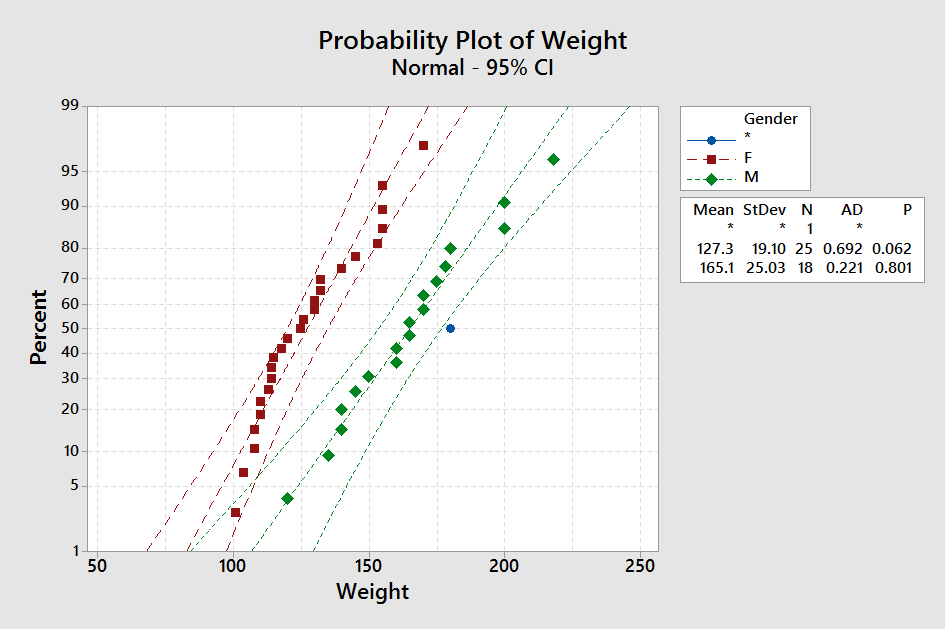
\includegraphics[scale=.4,keepaspectratio=true]{./project_files/probplot_weights-male-vs-female.png}
 % probplot_weights-male-vs-female.png: 945x629 pixel, 96dpi, 25.00x16.64 cm, bb=0 0 709 472
\end{figure}

    Next, we need to decide whether to use pooled variance or separate
variance. Since the size of each group is different and the standard
deviations are off by about 6 lbs, we will use the non-pooled t-test.

\begin{figure}[h!]
 \centering
 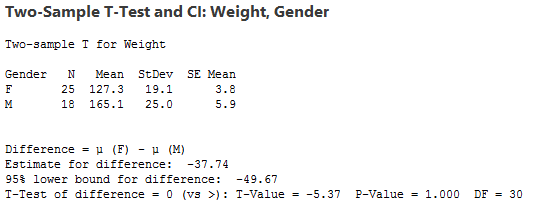
\includegraphics[scale=.7,keepaspectratio=true]{./project_files/2-sample_t-test_gender-weight.png}
 % 2-sample_t-test_gender-weight.png: 533x207 pixel, 96dpi, 14.10x5.48 cm, bb=0 0 400 155
\end{figure}


Since the p-value \textgreater{} \(\alpha = .01\), we cannot reject the
null hypothesis. We conclude that the mean weight of males is greater
than or equal to that of females.

    \subsubsection{Question 4}\label{question-4}

The paired t-test can be used to compare the difference between the
current weight and the ideal weight for each participant in the survey.

I believe that most people wish to lose weight, therefore I establish my
hypotheses:

\(H_0: \mu_d = \mu_{current} - \mu_{ideal} \le 0\)

\(H_a: \mu_d = \mu_{current} - \mu_{ideal} > 0\) 

\(\alpha = .015\)

degrees of freedom = 43 - 1 = 42

    \begin{Verbatim}[commandchars=\\\{\}]
{\color{incolor}In [{\color{incolor}72}]:} \PY{c}{\PYZsh{} compute mean difference}
         \PY{p}{(}\PY{n}{data}\PY{o}{.}\PY{n}{Weight} \PY{o}{\PYZhy{}} \PY{n}{data}\PY{p}{[}\PY{l+s}{\PYZdq{}}\PY{l+s}{Ideal\PYZhy{}weight}\PY{l+s}{\PYZdq{}}\PY{p}{]}\PY{p}{)}\PY{o}{.}\PY{n}{mean}\PY{p}{(}\PY{p}{)}
\end{Verbatim}

            \begin{Verbatim}[commandchars=\\\{\}]
{\color{outcolor}Out[{\color{outcolor}72}]:} 7.930232558139535
\end{Verbatim}
        
    \begin{Verbatim}[commandchars=\\\{\}]
{\color{incolor}In [{\color{incolor}75}]:} \PY{c}{\PYZsh{} compute std dev}
         \PY{p}{(}\PY{n}{data}\PY{o}{.}\PY{n}{Weight} \PY{o}{\PYZhy{}} \PY{n}{data}\PY{p}{[}\PY{l+s}{\PYZdq{}}\PY{l+s}{Ideal\PYZhy{}weight}\PY{l+s}{\PYZdq{}}\PY{p}{]}\PY{p}{)}\PY{o}{.}\PY{n}{std}\PY{p}{(}\PY{n}{ddof}\PY{o}{=}\PY{l+m+mi}{1}\PY{p}{)}
\end{Verbatim}

            \begin{Verbatim}[commandchars=\\\{\}]
{\color{outcolor}Out[{\color{outcolor}75}]:} 12.821847702888126
\end{Verbatim}
        
    \begin{figure}[h!]
 \centering
 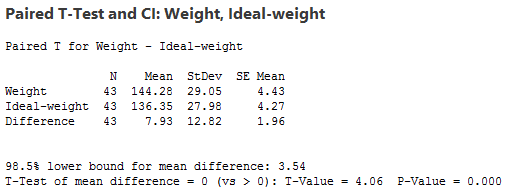
\includegraphics[scale=.7,keepaspectratio=true]{./project_files/paired-data_t-test_weight-vs-ideal-weight.png}
 % paired-data_t-test_weight-vs-ideal-weight.png: 509x194 pixel, 96dpi, 13.47x5.13 cm, bb=0 0 382 145
\end{figure}


p-value = 0.0000 \textless{} 0.015, so we can reject \(H_0\) and
conclude that people's ideal weight is less than their current weight.

    \subsubsection{Question 5}\label{question-5}

The data for this question is paired and is calling for a one-tailed
test. We already calculated the standard deviation in the previous
question, 12.8218.

\begin{figure}[h!]
 \centering
 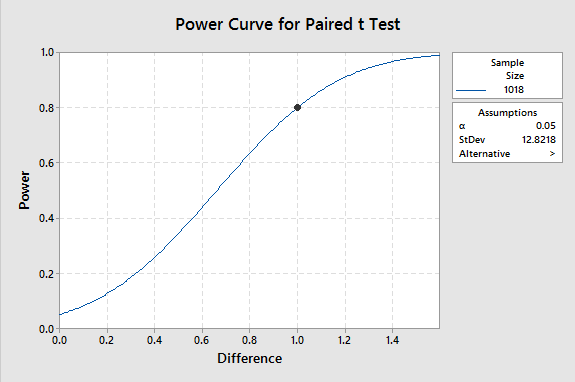
\includegraphics[scale=.7,keepaspectratio=true]{./project_files/pair-data_power-curve.png}
 % pair-data_power-curve.png: 575x382 pixel, 96dpi, 15.21x10.11 cm, bb=0 0 431 286
\end{figure}


Based on the power curve, we would need to sample 1018 students.

\newpage
    \subsubsection{Question 6}\label{question-6}

For the two qualitative variables, I chose gender and favorite sport. I
wanted to test if there was dependence between these two variables.
Since Hockey did not have any respondents, I excluded it from the table
since it didn't have any effect on the test.

\begin{longtable}[c]{@{}lllll@{}}
\toprule
& Football & Basketball & Other & Total\tabularnewline
\midrule
\endhead
Male & 5 & 4 & 9 & 18\tabularnewline
Female & 5 & 6 & 14 & 25\tabularnewline
Total & 10 & 10 & 23 & 43\tabularnewline
\bottomrule
\end{longtable}

\begin{figure}[h!]
 \centering
 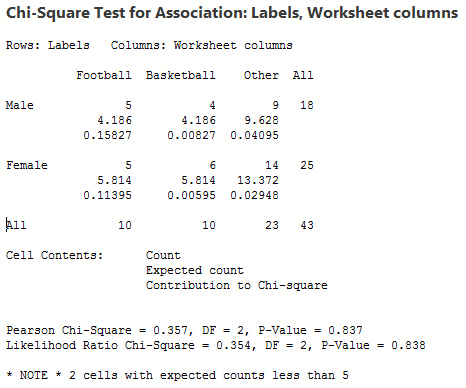
\includegraphics[scale=.7,keepaspectratio=true]{./project_files/chi-square-test_gender-vs-sports.png}
 % chi-square-test_gender-vs-sports.png: 466x388 pixel, 96dpi, 12.33x10.26 cm, bb=0 0 349 291
\end{figure}


The results of the Chi-square test indicate that we cannot reject the
null hypothesis that the values are independent. However, since there
are 2 cells (33.3\%) with expected count \textless{} 5, we cannot trust
the result.


    % Add a bibliography block to the postdoc
    
    
    
    \end{document}
